\documentclass{standalone}
\usepackage{tikz,lmodern,amssymb,xcolor}
\usetikzlibrary{calc}
\usepackage{knowledge}

\begin{document}

\begin{defn*}{Dot Product}
  \subsubsection*{Geometric}
  Let $ \vec{u}, \vec{v} \in \mathbb{R} ^{n}$ and let $\theta$ be the angle between the two (the one in the range $ \left[ 0, \pi \right]$), then we have the dot product: 
\[
	\vec{v}  \cdot  \vec{u} \stackrel{\mathtt{D}}{=} \left\Vert v \right\Vert \left\Vert u \right\Vert \cos  \left( \theta \right) 
\]
\begin{center}
	\newcommand{\tikzAngleOfLine}{\tikz@AngleOfLine}
	  \def\tikz@AngleOfLine(#1)(#2)#3{%
	  \pgfmathanglebetweenpoints{%
	    \pgfpointanchor{#1}{center}}{%
	    \pgfpointanchor{#2}{center}}
	  \pgfmathsetmacro{#3}{\pgfmathresult}%
	  }
	\newcommand{\tikzMarkAngle}[3]{
	\tikzAngleOfLine#1#2{\AngleStart}
	\tikzAngleOfLine#1#3{\AngleEnd}
	\draw #1+(\AngleStart:0.35cm) arc (\AngleStart:\AngleEnd:0.35cm);
	}
	\usetikzlibrary{patterns,decorations.pathreplacing}
	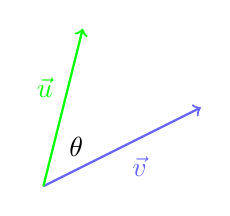
\begin{tikzpicture}
		\coordinate (A) at (2,1);
		\coordinate (B) at (.5,2);
		\coordinate (O) at (0,0);

		\draw[->,thick,blue!60!white] (0,0) -- +(A) node [midway,below right] {$\vec v$};
		\draw[->,thick,green] (0,0) -- +(B) node [midway,above left] {$\vec u$};
		\tikzMarkAngle{(O)}{(A)}{(B)}
		\node at ($(O)+(50:.65)$) {$\theta$};
	\end{tikzpicture}
	\hspace{1cm}
	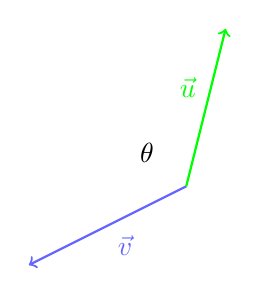
\begin{tikzpicture}
		\coordinate (A) at (-2,-1);
		\coordinate (B) at (.5,2);
		\coordinate (O) at (0,0);

		\draw[->,thick,blue!60!white] (0,0) -- +(A) node [midway,below right] {$\vec v$};
		\draw[->,thick,green] (0,0) -- +(B) node [midway,above left] {$\vec u$};
		\tikzMarkAngle{(O)}{(B)}{(A)}
		\node at ($(O)+(140:.65)$) {$\theta$};
	\end{tikzpicture}
\end{center}
\subsubsection*{Algebraic}
 Let $ u_{1} , u_{2} , \dotsc  , u_{n - 1} , u_{n}$ and $ v_{1} , v_{2} , \dotsc  , v_{n - 1} , v_{n}$ denote the components of $ \vec{u}$ and $ \vec{v}$ respectively, then we have:
\[
	\vec{v}  \cdot  \vec{u} \stackrel{\mathtt{D}}{=} \sum_{i=1}^{n} v_{i} u_{i}
\]



\end{defn*}

\end{document}
